\chapter{Première Version : Robot Réactif}



\section{Diagramme de Classes}

Le diagramme de classe est censé représenté la structure statique d'un système. Seulement comme dans GAMA tout est agent, les classes que nous manipulerons ici ne représentent en fait que des agent formalisés selon UML. Elles dérivent donc toutes de la classe "agent" nativement définie dans la documentation de GAMA. Nous ne représenterons pas cette classe dans nos diagrammes ici. 
Ci-dessous le diagramme de classe du modèle avec Robots Réactifs. 

\begin{figure}[h!]
	\begin{center}
		%taille de l'image en largeur
		%remplacer "width" par "height" pour régler la hauteur
		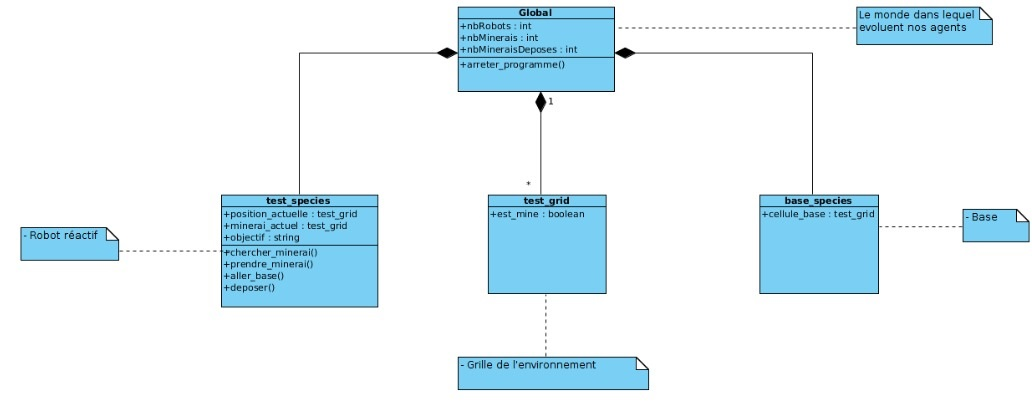
\includegraphics[width=500pt]{diagrammes/diagramme_classe_reactif}
	\end{center}
	%légende de l'image
	\caption{Diagramme de classe du robot réactif}
\end{figure}


Dans ce diagramme nous avons:

\begin{description}
	\item[Le Monde "global"] Il représente l'environnement dans lequel s'exécute la simulation. Il est lui même un agent et sert de conteneur a tous les autres agents du modèle, ce qui justifie la relation de composition qu'il partage avec toutes les autres classes. Comme son nom l'indique, il contient l'ensemble des variables et configurations globales du modèle et des expérimentations que nous ferons. 
	
	\item[La grille (les Cellules) "test\_grid"] Ce sont les cellules de la grille dans laquelle notre simulation se déroule. Chacune d'entre elle est dotée d'un attribut additionnel "est\_mine" qui permet de connaitre si la zone recouverte par la cellule contient ou non un minerai.
	
	\item[la Base "base\_species"] c'est l'agent qui représente la base de stockage des minerais. Il est associé à une des cellules de la grille choisie arbitrairement (ici cellule de la première ligne et de la premiere colonne) avec qui elle partage ainsi la même position. 
	
	\item[Les Robots Réactifs "test\_species"] C'est notre Robot collecteur, il est réactif mais pas "intelligent" puisqu'il n'a aucun moyen de savoir à priori où se trouve la base. Tout ce qu'il sait faire c'est se déplacer aléatoirement de voisins en voisins jusqu'à ce qu'il trouve la base dans sa zone de perception (cellule actuelle + cellules voisines).
\end{description}

\section{Diagramme d'Activités}

\begin{figure}[!h]
	\begin{center}
		%taille de l'image en largeur
		%remplacer "width" par "height" pour régler la hauteur
		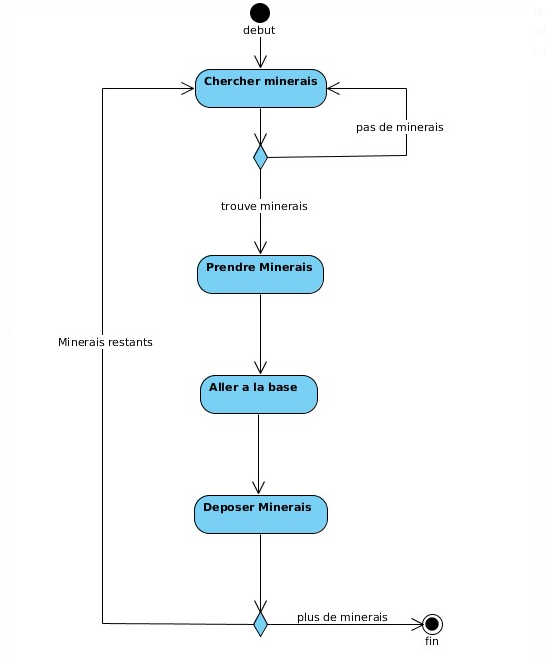
\includegraphics{diagrammes/diagramme_activites_reactif}
	\end{center}
	%légende de l'image
	\caption{Diagramme d'activités du robot réactif}
\end{figure}

Voici le diagramme d'activités du robot réactif. Ces activités correspondent à des réflexes de nos agents. Nous allons détailler chacune de ces activités.

\newpage

\subsection{Recherche de minerai [Chercher Minerais]}

Dans cette étape du scénario le robot vérifie d'abord si la cellule de grille (qui correspond à une zone) dans laquelle 
il se trouve contient un minerais. Sinon il cherche si les cellules voisines en contiennent. Si ni la cellule actuelle ni aucune de ses voisines ne contiennent de minerais alors le robot se déplace aléatoirement dans l'une des cellules voisines de la cellule actuelle pour y exécuter le même traitement au prochain pas de temps (cycle). Dans le cas contraire (il trouve un minerais) il passe à l'étape de collecte du minerais. \\
Cette étape du scénario est implémentée de la façon suivante : 
\begin{figure}[!h]
	\begin{center}
		%taille de l'image en largeur
		%remplacer "width" par "height" pour régler la hauteur
		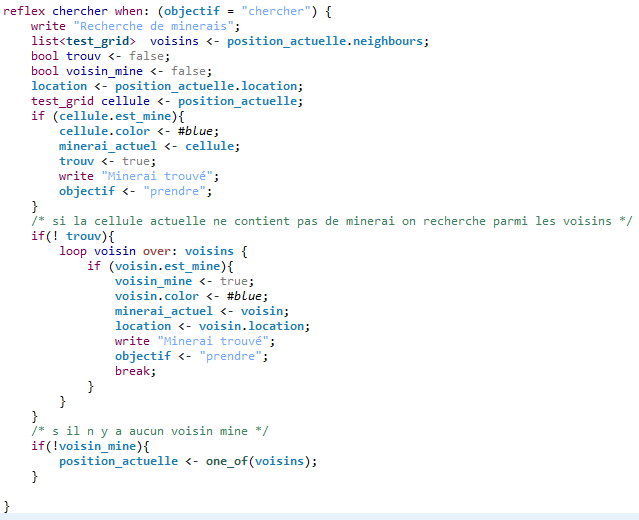
\includegraphics{code/chercher}
	\end{center}
	%légende de l'image
	\caption{Réflexe chercher}
\end{figure}

\subsection{Prise de minerai [Prendre Minerai]}

Cette étape ne se déclenche que quand le robot trouve un minerais dans l'une des cellules qu'il vient d'explorer. Durant cette etape le robot correspond a la collecte de minerais presénts dans la zone explorée. Cela correspond dans notre simulation à la modification d'un certain nombre d'attributs du robot et de la cellule de grille dans laquelle le minerais a été trouvé.\\
\newpage
Cette étape du scénario est implémentée de la façon suivante : 
\begin{figure}[!h]
	\begin{center}
		%taille de l'image en largeur
		%remplacer "width" par "height" pour régler la hauteur
		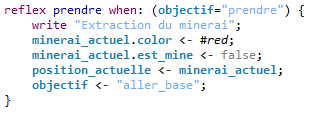
\includegraphics{code/prendre}
	\end{center}
	%légende de l'image
	\caption{Réflexe prendre}
\end{figure}

\subsection{Acheminement des minerais vers la base [Aller a la Base]}

Cette étape correspond à l'ensemble des déplacements aléatoires que le robot fait de voisins en voisins afin de trouver la base et d'y déposer le minerais collecté.\\ 
Cette étape du scénario est implémentée de la façon suivante : 
\begin{figure}[!h]
	\begin{center}
		%taille de l'image en largeur
		%remplacer "width" par "height" pour régler la hauteur
		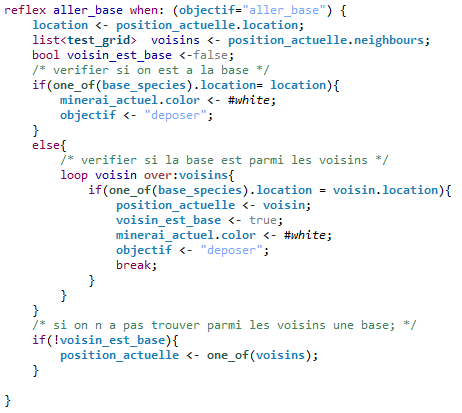
\includegraphics{code/aller_base_reactif}
	\end{center}
	%légende de l'image
	\caption{Réflexe aller\_base}
\end{figure}


\subsection{Dépôt de minerai}

Cette étape se déclenche une fois que le robot arrive a la base avec du minerais collecté. Elle correspond aussi (dans notre simulation) a la modification d'un ensemble d'attributs du robot qui montre que le dépôt a été bien fait et que le robot est à présent vide et prêt à aller rechercher d'autres minerais s'ils existent.\\
\newpage
Cette étape du scénario est implémentée de la façon suivante : 
\begin{figure}[!h]
	\begin{center}
		%taille de l'image en largeur
		%remplacer "width" par "height" pour régler la hauteur
		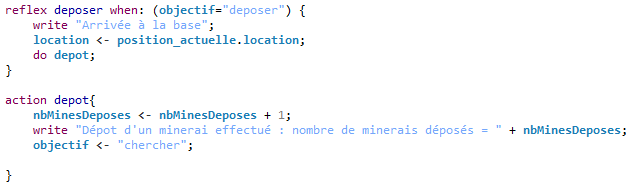
\includegraphics{code/deposer}
	\end{center}
	%légende de l'image
	\caption{Réflexe deposer}
\end{figure}


\subsection*{} 
Dans le diagramme d'activités ci-dessus les activités correspondent aux étapes que nous avons définies précédemment. Les seules nouveautés sont les deux nœuds de conditions:
\begin{itemize}
	\item La première se fait après l'étape "Chercher Minerais" et permet de tester si le robot a trouver un minerais dans sa zone de perception et ainsi 
	decider de s'il doit collecter et aller à la base ou tout simplement retourner à l'étape de recherche dans une autre zone de perception voisine.
	
	\item La seconde permet tester s'il existe encore des minerais dans l'environnement. Si c'est le cas le robot reprend tout le cycle d'activités à partir du début. Dans le cas contraire il s'arrête tout simplement.
\end{itemize}
